
% JuliaCon proceedings template
\documentclass{juliacon}
\setcounter{page}{1}
\bibliographystyle{juliacon}

\newcommand{\biochem}{BiochemicalAlgorithms.jl}{}
\newcommand{\bioviz}{BiochemicalVisualization.jl}{}
\newcommand{\ball}{BALL}{}
\newcommand{\ballFull}{Biochemical Algorithms Library }{}
\newcommand{\ballview}{BALLView}{}

\newcommand{\pdb}{PDB file}{}

\begin{document}

% **************GENERATED FILE, DO NOT EDIT**************

\title{Structure-based bioinformatics with BiochemicalAlgorithms.jl}

\author[1]{Jennifer Leclaire}
\author[1]{Thomas Kemmer}
\author[1]{Andreas Hildebrandt}
\affil[1]{Scientific Computing and Bioinformatics, Institute of Computer Science, Johannes Gutenberg-University Mainz}

\keywords{Julia, Structure-based bioinformatics, C++, BALL}

\hypersetup{
pdftitle = {Structure-based bioinformatics with BiochemicalAlgorithms.jl},
pdfsubject = {JuliaCon 2022 Proceedings},
pdfauthor = {Jennifer Leclaire, Thomas Kemmer, Andreas Hildebrandt},
pdfkeywords = {Julia, Structure-based bioinformatics, C++, BALL},
}



\maketitle




% A paper of about 5-10 pages +
% an abstract (at most 600 characters, written in plain English with no symbol nor formula)
% references [Author's guide]




\begin{abstract}
\biochem\ is framework for developing structure-based bioinformatics applications within the Julia ecosystem. Our library serves as a foundation providing rich functionality including file I/O, molecular modeling, molecular mechanics methods, and an accompanying visualization tool. \biochem\ is based on \ballFull (\ball), the largest open-source C++-framework of its kind. Our redesign emphasizes three design goals: ease of use, rapid application development, and functionality. Transitioning from C++ to Julia significantly simplified the realization of our design.
\end{abstract}





\section{Introduction}


The aim of structural bioinformatics is the analysis and targeted manipulation of three dimensional structures of biological macromolecules such as proteins and nucleic acids (RNA/DNA).
This research area combines and applies knowledge from diverse disciplines ranging from fundamental physical laws such as Newton's equation of motion to complex situations requiring in-depth knowledge of biochemistry and advanced numerical computing methodologies.



More precisely, molecular modeling techniques typically rely on molecular mechanics in which a molecular force fields is being used to compute the energy of the examining structure.  
Resulting applications include structure minimization, molecular dynamics (MD) simulations and molecular docking scenarios. The latter is inevitable for drug design because it computes the best configuration for a given protein and a ligand (the drug) and compute the binding affinity. 
The importance of molecular applications has been demonstrated during the Covid-19 pandemic. Tools for molecular modeling and in particular docking suites were attracting widespread interest again in order to model SARS-COV-2 proteins and running molecular docking simulations. 





\todo{Write about: Rational Drug Design economically important} 
Why do we have to run simulations on the computer? Why is it necessary to perform it on a computer? Example Protein Ligand Docking... As an example.

For more than 50 years researcher have been studying molecular functions of proteins. 
The first attempts date back to 1959, when Max Perutz and John Kendrew used X-ray crystallography to to solve the structure of hemoglobin. 

A vital aspect of this research field is the availability of molecular structure data, which was solved by the initialization of the protein data bank in 1972. Although it only contained 7 structures, it now provides 227.561 experimentally solved structures (dated on: \todo{check number of structures in pdb} ). With the rapid rise of computed structures 

software development in interdisciplinary research areas such as structural bioinformatics was, and still is, typically challenging.
Software packages for handling molecular structures and molecular applications are available for many years and can be rougly divided into open-source and closed-sourced tools. Most software packages were created from 1995 to 2010 and written in C++. Although this choice of programming language enables the required efficiency, it does not allow for rapid prototyping, which is why
some software packages provide an additional interface in a scripting language like Python. 
 \todo{Cite}

The tools were often only designed for one specific task e.g., implementation of a structure minimization algorithm, docking algorithm... \todo{cite single approaches}
One example for the latter is Schroedinger \todo{cite schroedinger}
~\cite{kohlbacher_ballrapid_2000}


\begin{itemize}
	\item docking algorithmus
	\item kraftfelder..
\end{itemize}
The development of software packages for structural bioinformatics remains a challenging task. 

Several packages already exist in Julia related to structural bioinformatics. Most prominently, the packages under the two Github communities \textit{Molecular Simulation in Julia} and \textit{BioJulia}, which puts an emphasis on sequential bioinformatics. 

\textit{Molly.jl} is an excellent package for molecular simulations written in Julia and is part of the \textit{Molecular Simulation in Julia} Github community \cite{Greener2024}. 
Additionally, \textit{ProtoSyn.jl} is an interesting approach to handle and manipulate oligopeptides but does not seem to be actively maintained any more (the last push is 10 months ago).

A platform from which molecular file formats can be read and write, the entire preprocessing pipeline can be integrated and the infrastructure for molecular mechanics are provided is still lacking. 
There remains a need for a basis from which software packages for handling molecular file formats and the proper preprocessing


To the best of our knowledge a comparable package for molecular analysis does not exist in Julia. Furthermore, the ongoing developments around the \ball project including the molecular viewer indicate a strong need for such a framework. 


Here, we present \biochem. We provide the basis for interesting analysis encompassing the entire molecular modeling pipeline:
\begin{itemize}
	\item Reading common data formats such as PDB, hin, mol and JSON
	\item Preprocessing the input by preparing the entire system ready to simulate.
	\item Molecular Mechanics such as AMBER ForceField
	\item (Output writing) such as JSON
\end{itemize}

\biochem is designed to be a platform from which other packages can be included.

\section{\ball --  \ballFull}
\label{sec:ball}


\begin{figure}[t]
	\centerline{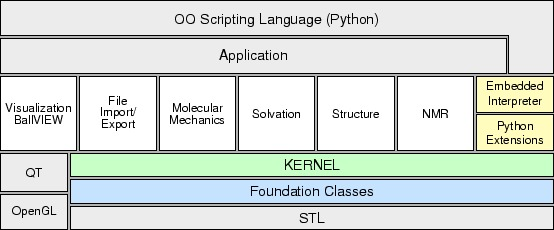
\includegraphics[width=0.5\textwidth]{gfx/BALL-architecture.jpeg}}
	\caption{\ball's architecture is structured in several layers. Upon the standard libary layer are the foundation classes and ontop of them the \texttt{KERNEL}. Several module extend the interface for visualization, file import and expoert, molecular mechanics, solvation, structure and NMR. The C++ written frameworkis extended by Python interface for fast scripting purposes. The figure was taken from the official \ball\ documentation \cite{BALLTutorial}.}
	\label{fig:ball_architecture}
\end{figure}


The main intention for the development of \ball\ as well as for \biochem\ is to generate a framework for rapid prototyping of molecular applications. This section summarizes the key concepts of \ball\ that motivated the design of our project \footnote{An in-depth description of the entire \ball\ framework is beyond the scope of this article. Confer the main publications~\cite{kohlbacher_ballrapid_2000, hildebrandt_ball_2010}  for more details.}\\
The initial work on the \ball\ project started in 1996, resulting in the C++-written library \ball\ and its accompanying molecular viewer, \textit{\ballview}. One reason for \ball's success lies in its sophisticated design; it employs an object-oriented approach with four design goals: \textit{ease of use}, \textit{robustness}, \textit{openness}, and \textit{functionality }
The object-oriented approach facilitates ease of use in combination with the well-documented and intuitive interfaces. As can be seen in Figure~\ref{fig:ball_architecture}, \ball's architecture is structured in several layers:
\begin{itemize}
	
	\item The standard template library (STL) forms its base.
	\item The foundation classes provide general data structures such as hash sets and mathematical objects (e.g., matrices, vectors,...). 
	\item The core consists of the \texttt{KERNEL} classes that contain data structures representing molecular entities.
	
	\item  The basic components represent fundamental functionalities placed atop of this core layer; exceptions include the visualization module that is based on Qt and Open GL \cite{Qt5,OpenGLWebsite}.
	\item Finally, the application layers can be used to develop custom applications or leverage existing tools. \\
\end{itemize}
Hildebrandt \textit{et al.} published an updated version in 2010, featuring  Python bindings alongside installation with the use of CMake as build system -- enhancements that improved usability and openness while allowing easier integration with external packages across different compilers/ operating systems \cite{hildebrandt_ball_2010}. \\

\ball's uniqueness stems from its rich functionality integrated in a single easily extensible open-source platform. Figure \ref{fig:ball_structure} illustrates how \texttt{KERNEL} classes form three frameworks: the general molecular framework, the protein framework, the nucleic acid framework -- all implemented through composite patterns \cite{gamma1994design}. More precisely, the composite class is the base class for all derived classes representing molecular entities such as \texttt{Atom}, \texttt{Protein}, etc. or container classes \texttt{System}, \texttt{AtomContainer}, and so on. \\ 

These frameworks form the basis for the functionalities of the basic components ranging from preprocessing tools (file import/export) to complex analyses (e.g., energy minimization/mapping) alongside advanced solvation methods. 
\ball\ is a well-tested library ensuring robustness of the provided functionalities. \\

\ball's robustness and well-designed structure has contributed significantly to its popularity -- \ball\ used to have one of the biggest user communities in this field.


\begin{figure}[t]
	\centerline{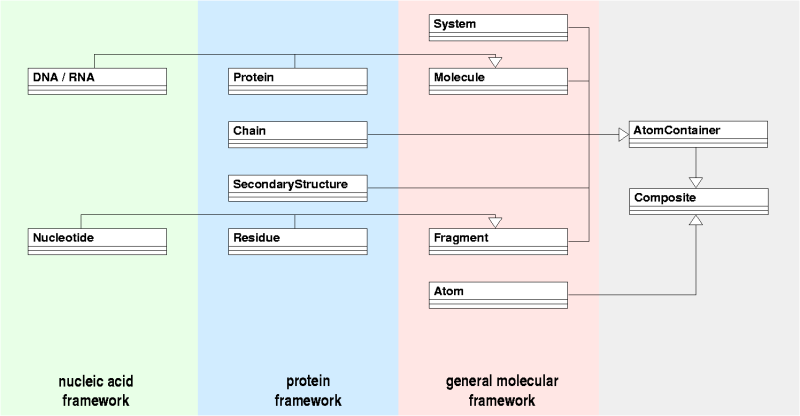
\includegraphics[width=0.5\textwidth]{gfx/KERNEL.png}}
	\caption{UML class diagram of the \texttt{KERNEL} classes. The \texttt{KERNEL} classes form three frameworks and are implemented using the composite pattern\cite{gamma1994design}. The figure was taken from the official \ball\ documentation \cite{BALLTutorial}.}
	\label{fig:ball_structure}
\end{figure}



\section{\biochem}
\label{sec:juliaball}
In this work, we sought to redesign the popular \ball package for molecular analysis and simulation. This section initially examines reasons for a redesign in Julia, followed by a description of the core implementation of \biochem closing with the benchmark results. 

\subsection{Reasons for a redesign or \textit{why Julia?}}

While the design goals and the need for an open-source framework with the rich functionality such as \ball's  is still present, the realization of the main design principles of \ball are highly dependent on the choice of the programming language. From today's perspective in particular with regard to its purpose as a platform for rapid application development~(RAD), the usage of C++ may be considered sub optimal. \\
As for many scientific software packages, the development times for applications play a crucial role for the acceptance and usability of the underlying software. For example, a great deal of time may have to be spend by installing the library with its dependencies. Although the CMake build system has been integrated in version 1.3, setting up the library is a highly non-trivial task. Additionally, the development times are massively influenced by the knowledge of the used programming language. As a low-level language, C++ is known to require more time to be learned compared to scripting languages such as Python \cite{Ousterhout1998}. 
Even with the additional Python bindings, the integration of new functionality is still not straightforward. In contrast, the implementation of new features is typically associated with the addition of massive amounts of boilerplate code. This applies to an even greater extent, in cases where portability to different platforms and compiler settings have to be supported. \\
Consequently, \ball itself can be considered as a textbook example for the two language problem, which is very common for scientific computing project. In the latter, the core functionality is often implemented in a low-level programming language, ensuring the required performance, while higher-level programming languages are used for user-friendly interfaces to the core functionalities. Julia is exactly developed for these situations \cite{Julia_what, Julia_accomplish}.\\ 
Nevertheless, it is important to keep in mind, that back in 1996 and still in 2010, C++ was the best choice for the implementation of \ball. \\
Switching our development from C++ to Julia has greatly simplified conforming the design goals denoted in Table~\ref{table1_design_goals}: 
\begin{itemize}
	\item Ease of use: \biochem's source code provides a better readability  as the usage of Julia does not produce so much boilerplate code compared to \ball. The integration of documentation, basic tutorials and test cases facilitates the introduction to \biochem, not to mention the trivial installation via Julia's Package manager. 
	
	\item Openness: Just like the installation, the integration of external tools to \biochem is straightforward. Our well documented framework allows the integration of own applications seamlessly. 
	
	\item Robustness: One of the strength of Julia is the integrated unit testing functionality allowing to test implemented code on the fly. \biochem has been carefully developed with accompanying test case for the core structures as well as for the functionalities ensuring non-faulty behavior using \texttt{TestItemRunner.jl}\cite{TestItemRunner}. Benchmark test cases are implemented in order to assess performance of typical tasks with the help of \texttt{BenchmarkTools.jl} and \texttt{Pkgbenchmark.jl} \cite{BenchmarkTools.jl-2016, PkgBenchmark}. The results of the benchmark study are described in section below. 
	
	\item Functionality: \biochem implements a set of standard data structures for molecular entities and already provides different functionalities based on these including import of structures stored in PDB, pubchem or hin files, molecular mechanics more precisely an interface for force fields and an Amber implementation, structure minimization algorithms. The interface are designed in a way that facilitates adoption e.g., implementation fo an own force field or changing an optimizer for the structure minimization. 
\end{itemize}

\subsection{The core representation}
In addition to the four original design goals, we sought to make \biochem comparable in performance to \ball. When working with structural data of molecular entities such as proteins, or nucleic acid molecules (DNA/RNA), the representation of atoms play an important role. \\
More precisely, we decided to put the \texttt{System} at the center of every application in \biochem. If the system is not defined explicitly, it will be generated by default. As shown in Figure~\ref{fig:biochem_uml}, the system contains data structures for the representation of atoms and bonds as soon as they are generated explicitly (see code listing ~\ref{lst:code-water})  or populated by reading files (see code listing ~\ref{lst:rmsd-and-amber}).  Other molecular data structures will only be generated on demand. \\
The representation of an atom with their position, velocity and force contributes substantially to the efficiency of the entire framework. Therefore, careful attention has been given to the implementation of the underlying data structure. Due to its popularity and intuitive usage, a preliminary attempt consisted of a representation using \texttt{DataFrames.jl} \cite{Bouchet-Valat2023}. However, we decided to move to a costume implementation of the \texttt{Tables.jl} interface \cite{BouchetValat2018} as initial benchmarks indicated a better performance (data not shown). \\
\todo{Tables interface allows to be converted to BioStructures.jl stuff and so on}
The Table~\ref{table2_benchmark} lists the results of a benchmark study comparing the time needed for typical core functionalities in \ball and \biochem. It is evident \biochem is on par with its C++ predecessor.
\begin{figure*}[t]
	\centerline{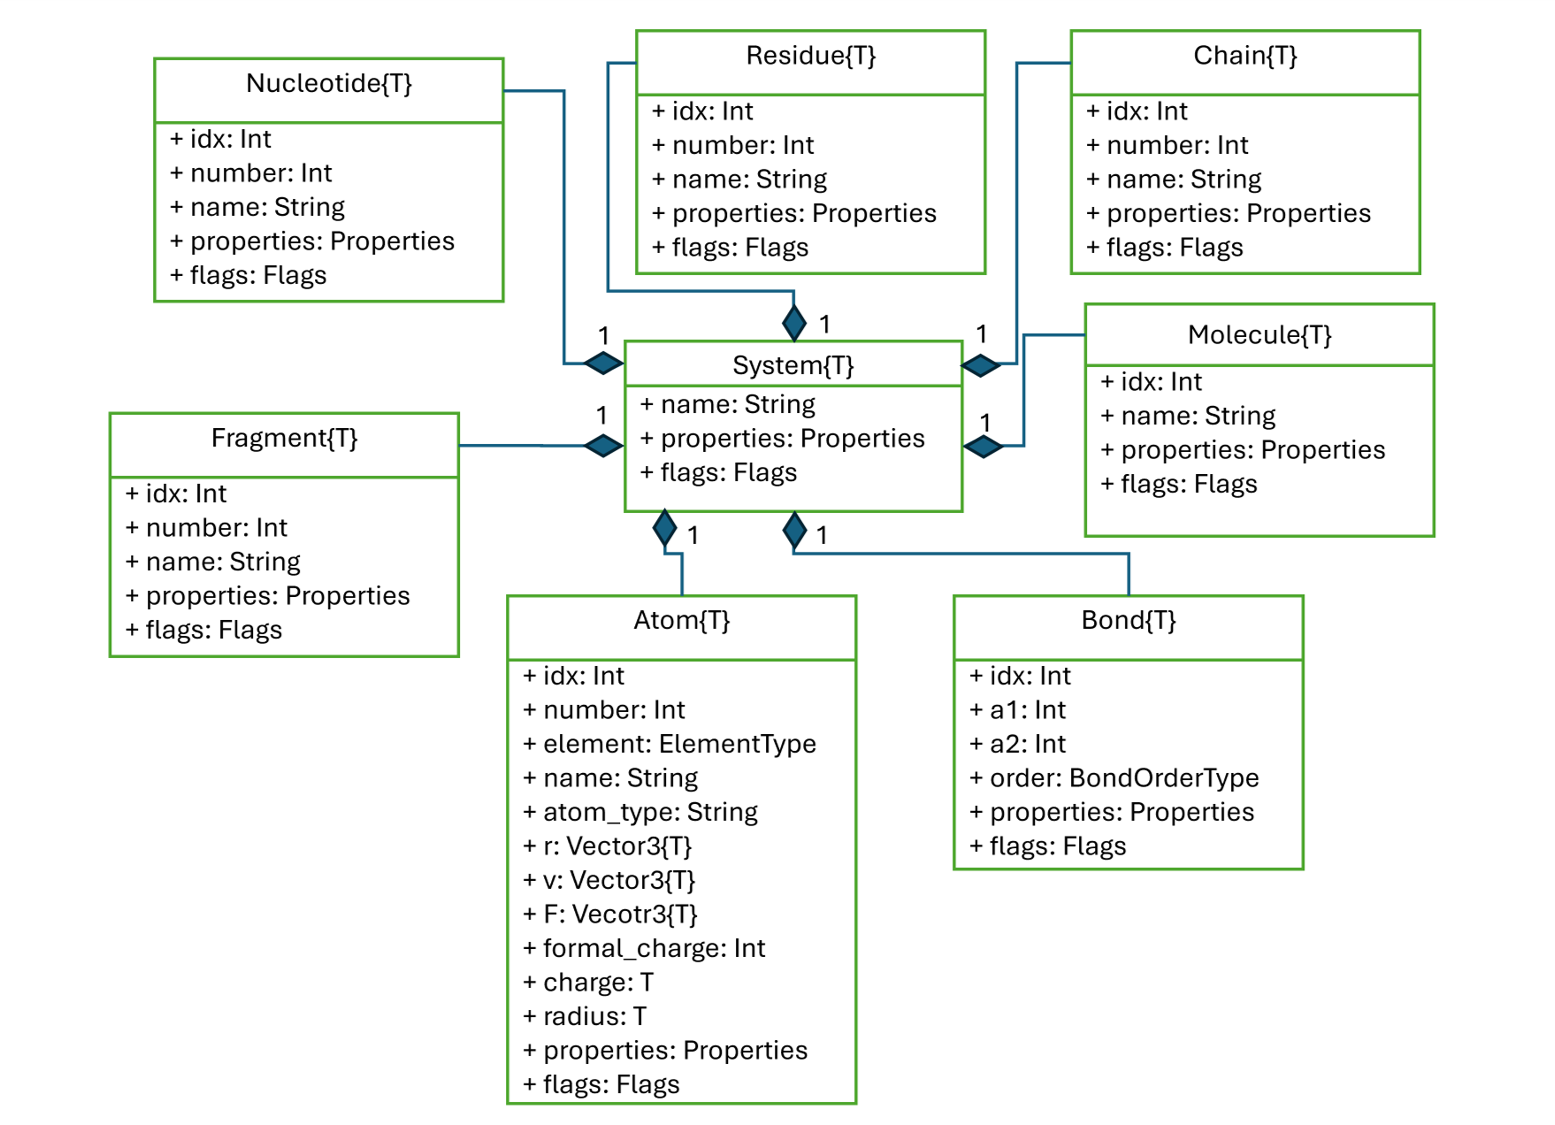
\includegraphics[width=15cm]{gfx/uml.png}}
	\caption{UML-Diagramm of the core of \biochem . In the center resides the \texttt{System} interface. All other functionalities are grouped around that core piece. Only the most important functionalities of each class are  shown.}
	\label{fig:biochem_uml}
\end{figure*}

\begin{table}
	\tbl{Example tasks and the required time}{
		\begin{tabular}{|l|c|c|}\hline
			Description & \ball & \biochem \\
			tba & tba & tba\\hline
			tba & tba & tba \\\hline
		tba	& tbal & tba \\ \hline
	\end{tabular}}
\label{table2_benchmark}
\end{table}
\section{Applications}

The functionality and usability of \biochem is best demonstrated with examples. We chose three small scenarios, we begin with a simple example to show how some of the core structures can be created and used. Then we had over to a more complex example where we want to compare two different configurations of the same molecule. Finally, we want to demonstrate the elegance of Julia written code in comparison to C++. In the last application, we briefly introduce the accompanying visualization tool \bioviz that has been developed alongside the \biochem framework.

\subsection{Generating a water molecule}

The class diagramm in Figure~\ref{fig:biochem_uml} shows the core of \biochem. The interface is intuitively designed and the interactions with the components are straightforward as can be seen in code listing~\ref{lst:code-water}. The center of an application is the \texttt{System}. If no such system is explicitely created a default system is generated. Atoms can be created and the corresponding bonds and will automatically be part of the defined system. The names of the classes for the molecular entities and related functionalities were carefully chosen to be as intuitive as possible. The resulting system with the contained water molecule can be visualized via the visualization tool \bioviz. See Figure~\ref*{fig:biochem_water} and the following sections for more details. 
\begin{lstlisting}[
language = Julia, 
numbers=left, 
label={lst:code-water}, 
caption={Intuitive usage of \biochem core components}
]
using BiochemicalAlgorithms
using BiochemicalVisualization

sys = System() 
h2o = Molecule(sys)

o1 = Atom(h2o, 1, Elements.O)
h1 = Atom(h2o, 2, Elements.H)
h2 = Atom(h2o, 3, Elements.H)

h1.r = [1, 0, 0]
h2.r = [cos(deg2rad(105)), sin(deg2rad(105)), 0]

Bond(h2o, o1.idx, h1.idx, BondOrder.Single)
Bond(h2o, o1.idx, h2.idx, BondOrder.Single)

println("Number of atoms: ", natoms(h2o))
println("Number of bonds: ", nbonds(h2o))

ball_and_stick(sys)	
stick(sys)
van_der_waals(sys)
\end{lstlisting}


\subsection{RMSD computation and Application of Amber}

A very common task in structural analysis is the comparison of two or more structures. The following example will demonstrate the entire molecular pipeline. First, the two pdb files are loaded into a system container. Compared to the previous example, the variable \texttt{sys} represent a \texttt{Vector} of \texttt{Systems} instead of a single system. The systems are preprocessed with the \texttt{FragmentDB}, a database containing known fragments of molecules. The preprocessing steps include the normalization of different naming standards, the reconstruction of missing parts of the molecules and the creation of bonds, since pdb format usually contain no or incomplete bond information.  After the preprocessing, the molecular structures are each applied to a molecular force field and here the amber energy of the systems are computed. The structures studied in this example are different configuration of the same molecule and can be mapped onto each other. Before and after the mapping the RMSD is computed and displayed.  \\
This example demonstrates the rich functionality of \biochem by just a few lines of code. The steps that were carefully taken to prepare the systems are shown in Figure\ref{fig:biochem_visualization}.
\begin{lstlisting}[
    language = Julia, 
    numbers=left, 
    label={lst:rmsd-and-amber}, 
    caption={Comparison and mapping of two similar structures}
]
sys = load_pdb.(["data/arnd1.pdb", 
				 "data/arnd2.pdb"])

fdb = FragmentDB()
normalize_names!.(sys, Ref(fdb))
reconstruct_fragments!.(sys, Ref(fdb))
build_bonds!.(sys, Ref(fdb))

println.(sys)

compute_energy.(AmberFF.(sys), verbose=true)

println("RMSD before mapping: ", 
		compute_rmsd(sys[1], sys[2]))

map_rigid!(sys[1], sys[2])

println("RMSD after mapping: ", 
		compute_rmsd(sys[1], sys[2]))
\end{lstlisting}

\todo{output?}
\subsection{A trivial comparison between C++ and Julia}

The verbose nature of C++ comes apparent in a simple task. A typical situation in molecular simulation is to find out, which atoms are in a certain proximity of each other. As these atoms can exert interactions, which are important for the stability of a structure configuration. We would solve this task with advanced data structures such as a hash grids. However, for simplicity, we consider the following task: We want to count the contacts between two separate molecules, that are in close proximity. We will define a contact, if the distance between two carbon atoms $C_\beta$ atoms is smaller than $6$\AA. \\

The code listing below shows the solution for the task in C++. It is important to note here, that due to readability, the necessary includes for this even short code snippet are not shown. Using two nested for-loops, possible $C_\beta$ atoms are searched, whose distance from each other is computed in the next step. \\
In contrast, with \biochem this task is solved much
\begin{figure*}
\begin{lstlisting}[
	language = C++, 
	numbers=left, 
	label={lst:code-c++}, 
	caption={The resulting C++ code for the example task consist of a lot of boilerplate code.}
	]
int count_contacts(const AtomContainer& ac1, const AtomContainer& ac2, double thres = 6.0) {
	auto contacts = 0;
	for(auto ait1 = ac1.beginAtom(); +ait1; ++ait1) {
		if(ait1->getName() != "CB")
		continue;
		
		for(auto ait2 = ac2.beginAtom(); +ait2; ++ait2) {
			if(ait2->getName() != "CB")
			continue;
			
			auto dist = ait1->getPosition().getDistance(ait2->getPosition());
			if(dist <= thres) {
				contacts++;
			}
		}
	}
	return contacts;
}
\end{lstlisting}
\end{figure*}


\begin{figure*}
\begin{lstlisting}[
	language = Julia, 
	numbers=left, 
	label={lst:code-task-julia}, 
	caption={The resulting Julia code for the example task is much more elegant.}
	]
using BiochemicalAlgorithms 
	
function filter_cbeta(ac::AbstractAtomContainer{Float32})
	(atom for atom in atoms(ac) if atom.name == "CB")
end
	
function is_in_contact(r1::Vector3{Float32}, r2::Vector3{Float32})
	distance(r1, r2) <= 6
end
	
function count_contacts(ac1::AbstractAtomContainer{Float32}, ac2::AbstractAtomContainer{Float32})
	count( t -> is_in_contact(t...), ((a1.r, a2.r) for a1 in filter_cbeta(ac1), a2 in filter_cbeta(ac2)))
end
\end{lstlisting}
\end{figure*}

\subsection{Visualization using \bioviz}

A key feature of \biochem is the visualization tool \textit{\bioviz} that
has been developed alongside the main framework. As shown in Figure~\ref{fig:biochem_water} \ \bioviz currently supports three different representation of atomic structures, namely \texttt{ball-and-stick}, \texttt{van-der-Waals} and \texttt{stick} (cf. code listing~\ref{lst:code-water}).

When dealing with three dimensional structures of macromolecules, visualization plays an important role for supporting the development of insights into molecular functions. The possibility to visualize and interactively modify the representations provides great support during modelling scenarios. For instance, the tool has been used to visualize different steps from code listing~\ref{lst:rmsd-and-amber}. The first image left represent the raw input read from the underlying pdb file, the image in the middle shows the same input after preprocession it with the fragment data base (lines4-7). Finally, the mapping of both structures is shown in the image on the left. As can be seen, the structures do not match perfectly onto each other. 

Even this rather simple example already demonstrates the advantage of a visual representation that can be modified and manipulated in context of modelling scenarios and how the visualization supports the development of knowledge of molecular functions.

 \begin{figure*}[t]
	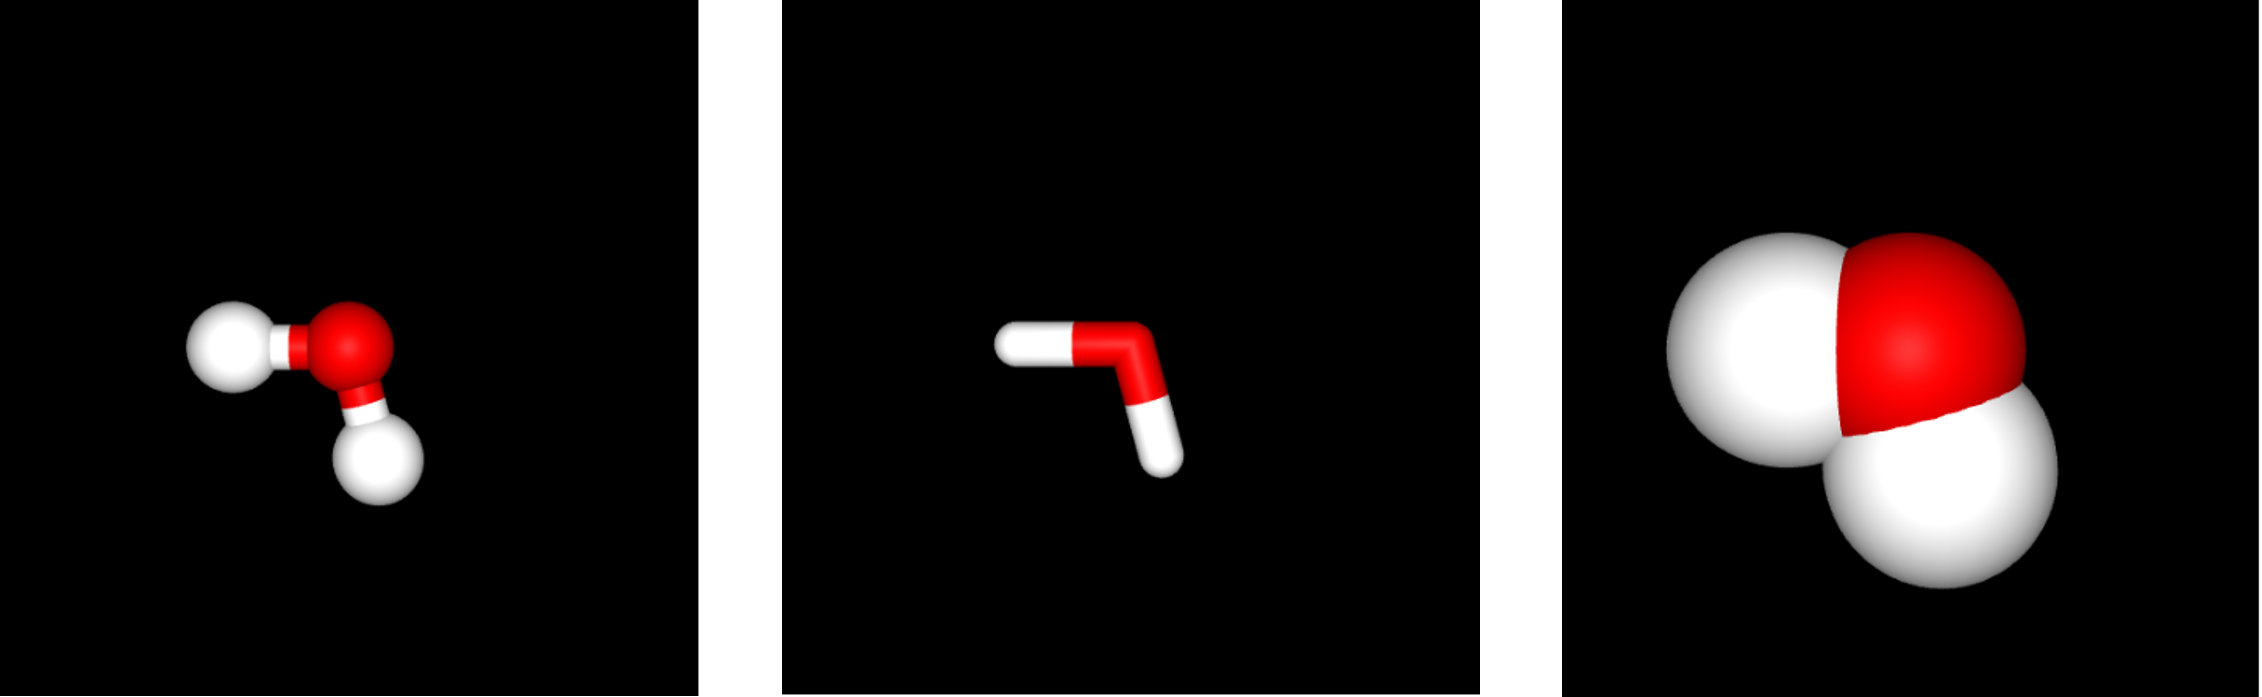
\includegraphics[width=18cm]{gfx/biovis-2.png}
	\caption{\bioviz supports three models:  \texttt{ball-and-stick} \textit{(left)}, \texttt{stick} \textit{(center)} and \texttt{van-der-waals} \textit{(right)} representation of the water molecule as generated by the code listing~\ref{lst:code-water}.}
	\label{fig:biochem_water}
\end{figure*}

\begin{figure*}[t]
	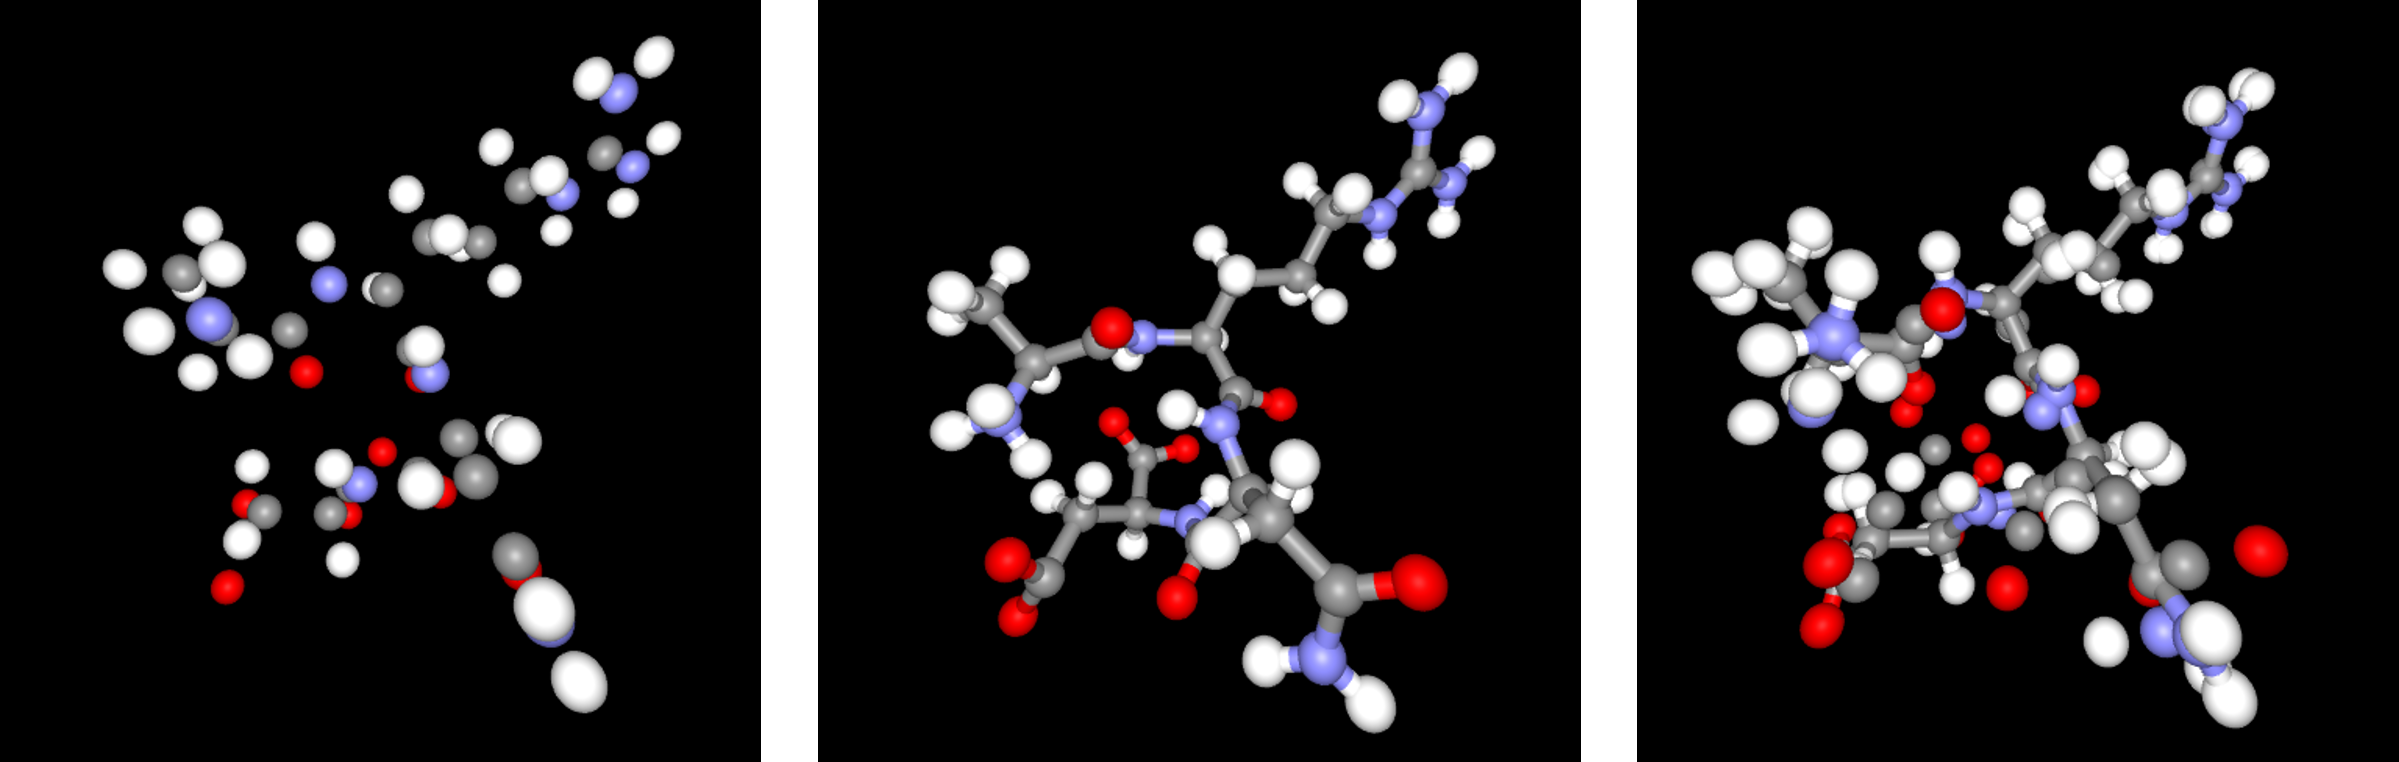
\includegraphics[width=18cm]{gfx/biovis.png}
	\caption{The \texttt{ball-and-stick}-representation of the code listing~\ref{lst:rmsd-and-amber}. The first molecule without preprocessing (\textit{left}) and after preprocessing (\textit{center}). Finally, the two structures are superposed (\textit{right}).}
	\label{fig:biochem_visualization}
\end{figure*}

\section{Conclusion}

We have presented a single and modern platform for the rapid application development of molecular structure analysis and simulations. While other Julia packages focused either on a single task like the manipulation of peptides or molecular dynamic simulations, \biochem serves as framework for exploration studies of structure or the proper initialization of structures for molecular simulations through the usage of the fragmentDB. Like its C++ predecessor, \biochem provides a robust but flexible core with additional functionalities. More precisely, the core has been carefully designed using a costume realization of the \texttt{Tables.jl}-interface. Thereby, our platform 
\begin{itemize}
	\item can be integrated to other tools using the tables interface
	\item fits into julia mol sim or BioJulia
	\item Achievement: \biochem allows the rapid prototyping of molecular analysis 
	\item Meaning of achievement: interface is so flexible that parts can be interchanged or it is easy to write your own tool not to take care of proper initialization if you want to implement a molecular force field 
	\item NOVELTY: Do we have one? 
	\item We believe that \biochem will be very helpful for scientist who want to do structural bioinformatics and don't know much about....additionally: visualization
	\item \biochem already provides basic functionalities and interfaces for molecular mechanics but much is still to be done e.g., implementation of a docking interface, implementation of other force fields... we still have to do a lot of stuff to be feature-complete to \ball
	\item 
\end{itemize}



\section*{Acknowledgements}

Parts of this research were conducted using the supercomputer MOGON NHR and/or advisory services offered by Johannes Gutenberg University Mainz (hpc.uni-mainz.de), which is a member of the AHRP (Alliance for High Performance Computing in Rhineland Palatinate,  www.ahrp.info) and the Gauss Alliance e.V.

The authors gratefully acknowledge the computing time granted on the supercomputer MOGON NHR at Johannes Gutenberg University Mainz (hpc.uni-mainz.de).

\bibliography{ref}
\end{document}

% Inspired by the International Journal of Computer Applications template
